\documentclass[table,serif,mathserif,professionalfont,aspectratio=169]{beamer}

\mode<presentation>
{
  \usetheme{CambridgeUS}
  \setbeamercolor{item projected}{bg=darkred}
  \setbeamertemplate{enumerate items}[default]
  \setbeamertemplate{navigation symbols}{}
  \setbeamertemplate{itemize item}{-}
  \setbeamertemplate{itemize subitem}[triangle]
  \setbeamercovered{transparent}
  \setbeamercolor{block title}{fg=darkred}
  \setbeamercolor{local structure}{parent=alerted text}
}
\addtobeamertemplate{block begin}{\setbeamercolor{local structure}{parent=structure}}{}

\usepackage[english]{babel}
\usepackage{amssymb}
\usepackage{mathcmd}
\usepackage{nicefrac}
\usepackage{booktabs}
\usepackage{graphicx}
\usepackage{siunitx}
\usepackage{bbm}
\graphicspath{{./../../plots/}{./../../pictures/}}

%\usepackage{courier}
%\usepackage{times}
% The non-standard packages arev and bera define fonts which look nicely for
% projection, you might want to try them instead of Times/Helvetica/Courier.
% Use the

%%%%%%%%%%%%%%%%%%%%%%%%%%%%%%%%%%%%%%%%%%%%%%%%%%%%%%%%%%%%%%%%%%%%%%%%
\usepackage{pxfonts} % Or palatino or mathpazo
\usepackage{eulervm}
\linespread{1.05}
%%%%%%%%%%%%%%%%%%%%%%%%%%%%%%%%%%%%%%%%%%%%%%%%%%%%%%%%%%%%%%%%%%%%%%%%
\usepackage[T1]{fontenc}
% Or whatever. Note that the encoding and the font should match. If T1
% does not look nice, try deleting the line with the fontenc.
\usepackage{hyperref}

\newcommand{\prob}[1]{\ensuremath{\mathbb{P}\left(  #1 \right)}}
\newcommand{\mean}[1]{\ensuremath{\mathbb{E}\left(  #1 \right)}}
\newcommand\independent{\protect\mathpalette{\protect\independenT}{\perp}}
\newcommand{\menquote}[1]{\ensuremath{\text{\textquotedbl} #1 \text{\textquotedbl}}}
\def\independenT#1#2{\mathrel{\rlap{\(#1#2\)}\mkern2mu{#1#2}}}

%\setbeamerfont{alerted text}{series=\scshape}

\title[Data-driven modelling for inbound air traffic]{1-D gas models of air traffic at some major European airports}
\subtitle{Data-driven modelling and validation of the inbound flow}

\author[CL]{Carlo Lancia \inst{1} \and Guglielmo Lulli \inst{2}}

\institute[Leiden Univ.\ MI]{\inst{1} Leiden Univ.\ Math.\ Inst., \inst{2} Lancaster Univ.}

\date[ECSO 2017]{GSSI, L'Aquila, October 21, 2016}
% - Either use conference name or its abbreviation.
% - Not really informative to the audience, more for people (including
%   yourself) who are reading the slides online

% \usepackage{hyperref}
% \subject{Cutoff phenomenon for finite Markov chains}
% This is only inserted into the PDF information catalog. Can be left
% out.

% \AtBeginSection[]
% {
%   \begin{frame}<beamer>
%     \frametitle{Outline}
%     \tableofcontents[currentsection,hideothersubsections]
%   \end{frame}
% }
% Use this if you do want the table of contents to pop up at
% the beginning of each subsection.

% \pgfdeclareimage[height=2em,interpolate=true]{ntnulogotext}{foo}
% If you want to include a different logo on the title page
% only (e.g. a combined logo of different institutions), you
% can use this command.

% -------------------------------------
% \includeonlyframes{current}
% -------------------------------------

\begin{document}

\maketitle
% You can use \maketitle to create the titlepage,
% or \compressedtitle to create a more compact titlepage
% with the look of the other pages in compress style

% \begin{frame}
%   \titlepage
% \end{frame}
% Or you can call the titlepage command in a frame environment

% \begin{frame}<beamer>[label=current]
%   \frametitle{Outline}
%   \tableofcontents[hideallsubsections]
% \end{frame}

  \begin{frame}[t]\frametitle{Motivation}
      \begin{alertblock}{Single-server queue model with deterministic service time}
        \centering
        \begin{columns}
          \begin{column}{.495\textwidth}
            \centering
            \includegraphics[width=\textwidth]{HeathrowFit_01}\\
            {\scriptsize Poissonian Arrivals}
          \end{column}
          \begin{column}{.495\textwidth}
            \centering
            \includegraphics[width=\textwidth]{HeathrowFit_02}\\
            {\scriptsize Pre-Scheduled Random Arrivals}
          \end{column}
        \end{columns}
      \end{alertblock}
  \end{frame}

  \begin{frame}[t]\frametitle{1-D Gas models}
    Gigi
  \end{frame}

  \begin{frame}[t]\frametitle{Data description}
    \begin{table}[tbp]
      \centering
      \vfill
      \begin{tabular}{lcr}
        \toprule
        airport name & ICAO code & inbound flights\\
        \midrule
        Frankfurt am Main  & EDDF & 62531 \\
        London Gatwick     & EGKK & 22119 \\
        London Heathrow    & EGLL & 61880 \\
        London Stansted    & EGSS & 22119 \\
        Amsterdam Schiphol & EHAM & 55482 \\
        Roma Fiumicino     & LIRF & 45256 \\
        \bottomrule
      \end{tabular}
    \end{table}
    \vfill
  \end{frame}

  \begin{frame}[t]\frametitle{Poisson and PSRA-like arrival stream}
    Something
  \end{frame}

  \begin{frame}[t]\frametitle{Data querying}
      \begin{columns}
        \begin{column}{.4\textwidth}
          \begin{itemize}
            \item Terminal Control centrally manages and regulates inbound traffic
            \item The action of Terminal Control reflects a strong interaction between aircraft
            \item We want to focus on the time until reaching Terminal Control (red airspace)
            \item A good proxy for this is the time of first descent below 24.000 feet of altitude (FL240)
          \end{itemize}
        \end{column}
        \begin{column}{.6\textwidth}
          \includegraphics[width=\textwidth]{LondonACC}
        \end{column}
      \end{columns}
  \end{frame}

  \begin{frame}[t]\frametitle{Time series analysis}
    \begin{alertblock}{Frankfurt, Amsterdam, Rome}
      \centering
      \includegraphics[width=.8\textwidth]{OtherAirports}
    \end{alertblock}
  \end{frame}

  \begin{frame}[t]\frametitle{Time series analysis}
    \begin{alertblock}{Heathrow, Gatwick, Stansted}
      \centering
      \includegraphics[width=.8\textwidth]{LondonAirports}
    \end{alertblock}
  \end{frame}

  \begin{frame}[t]\frametitle{Analysis of interarrivals}
      Gigi
  \end{frame}

  \begin{frame}[t]\frametitle{Construction of non-homogeneneous Poisson process}
    \centering
    \includegraphics[width=.9\textwidth]{Poisson_AllAirports}
  \end{frame}

  \begin{frame}[t]\frametitle{Arrivals are actually correlated}
    \begin{alertblock}{Correlations from M3 data}
      \centering
      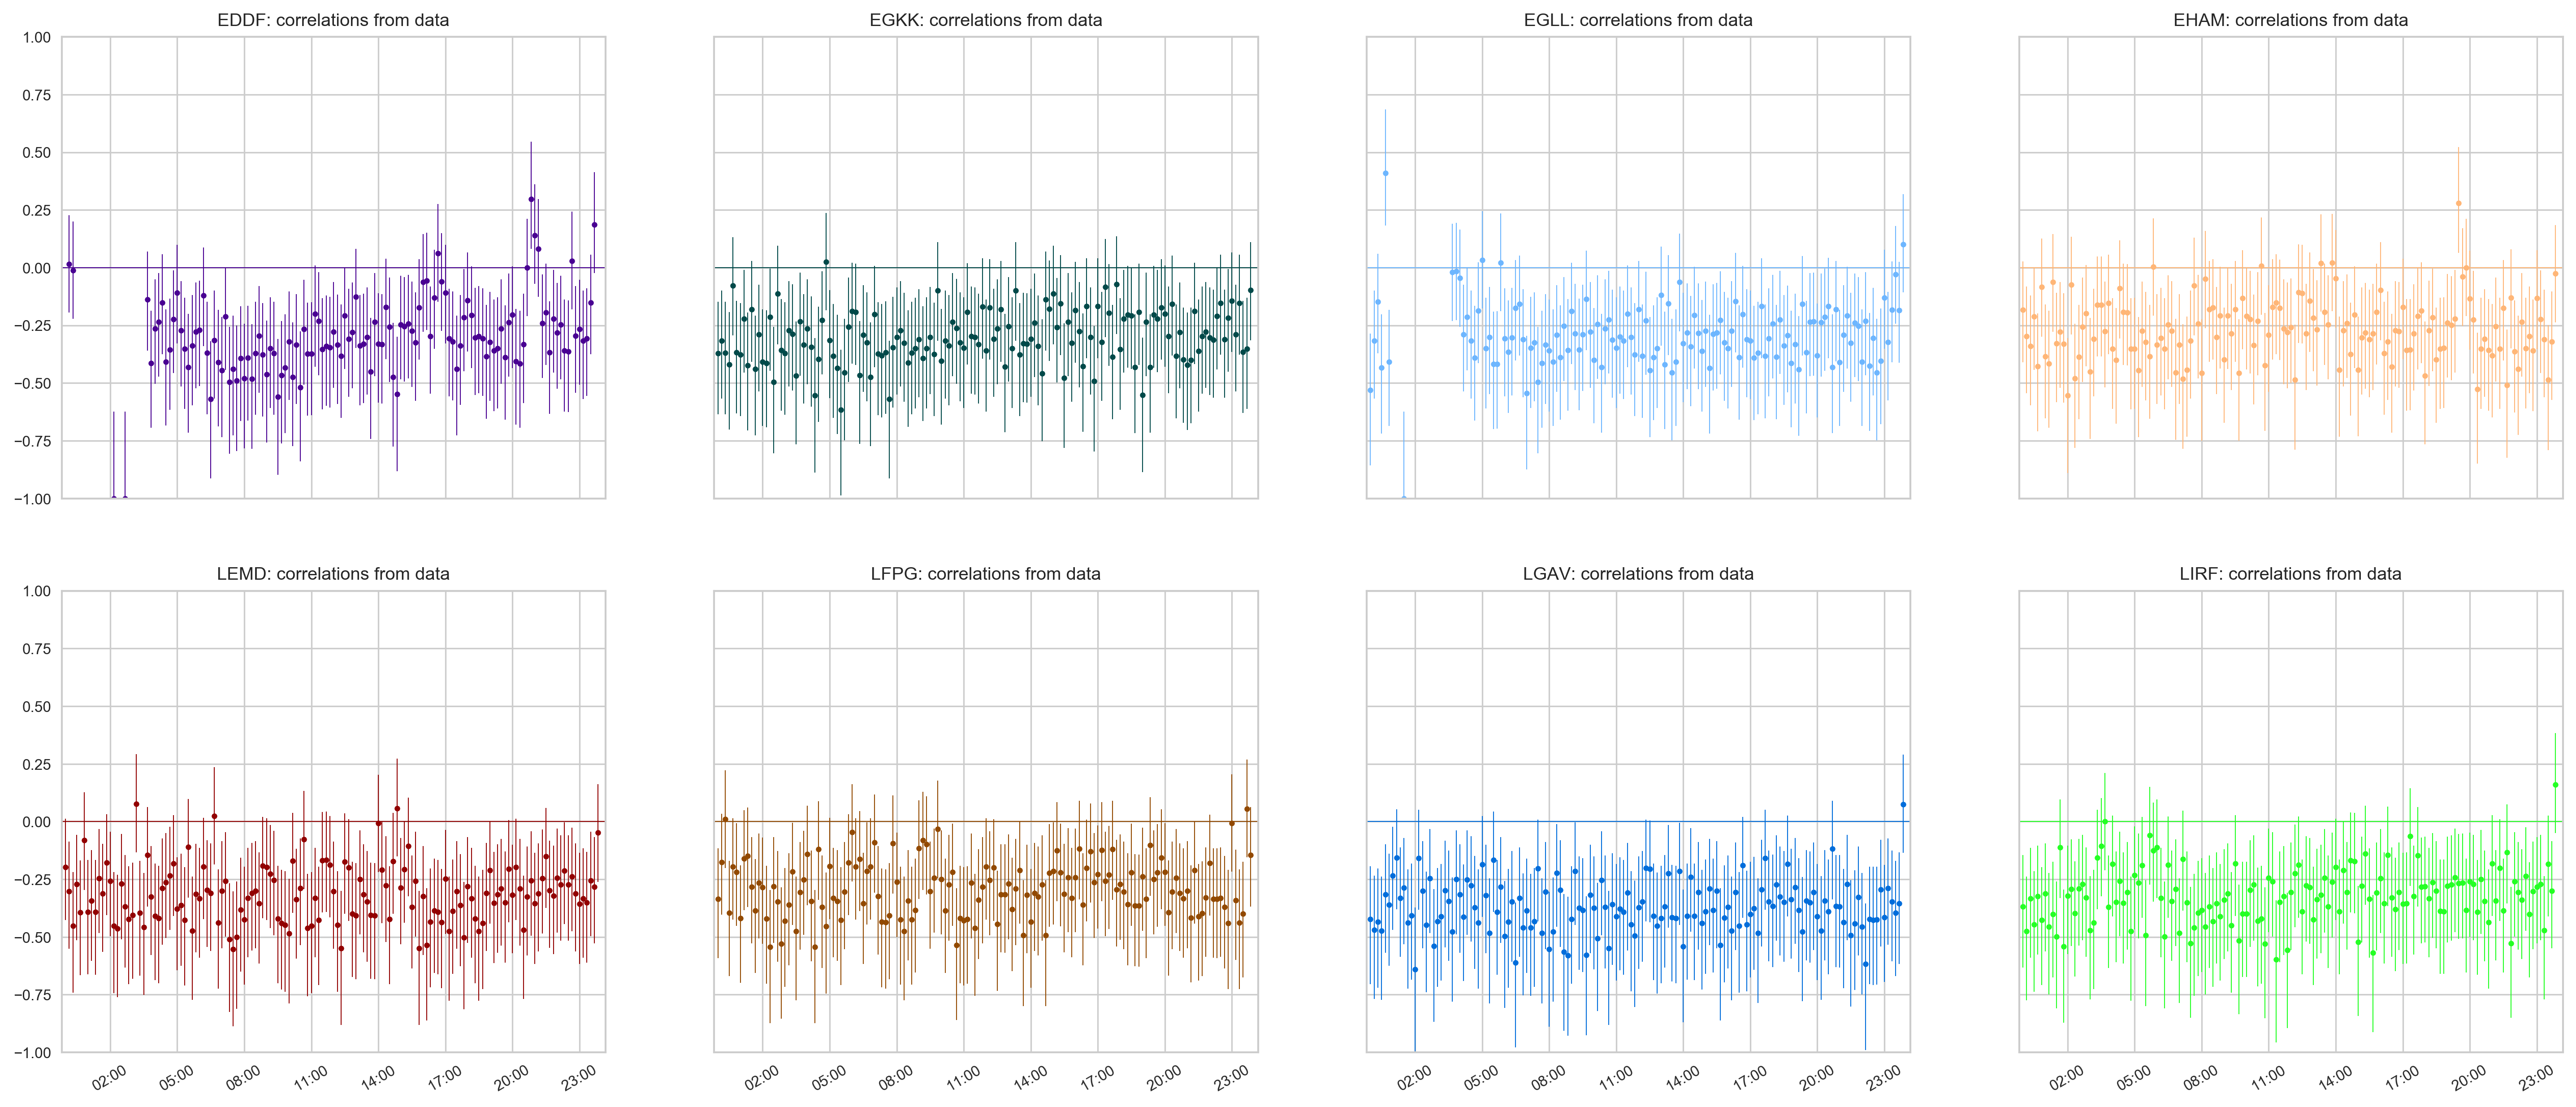
\includegraphics[width=.6\textwidth]{correlations_true}
    \end{alertblock}
  \end{frame}

  \begin{frame}[t]\frametitle{Definition of PSRA-like stream}
    Gigi
  \end{frame}

  \begin{frame}[t]\frametitle{PSRA-like arrivals are correlated}
      \begin{alertblock}{Correlations from PSRA}
        \centering
        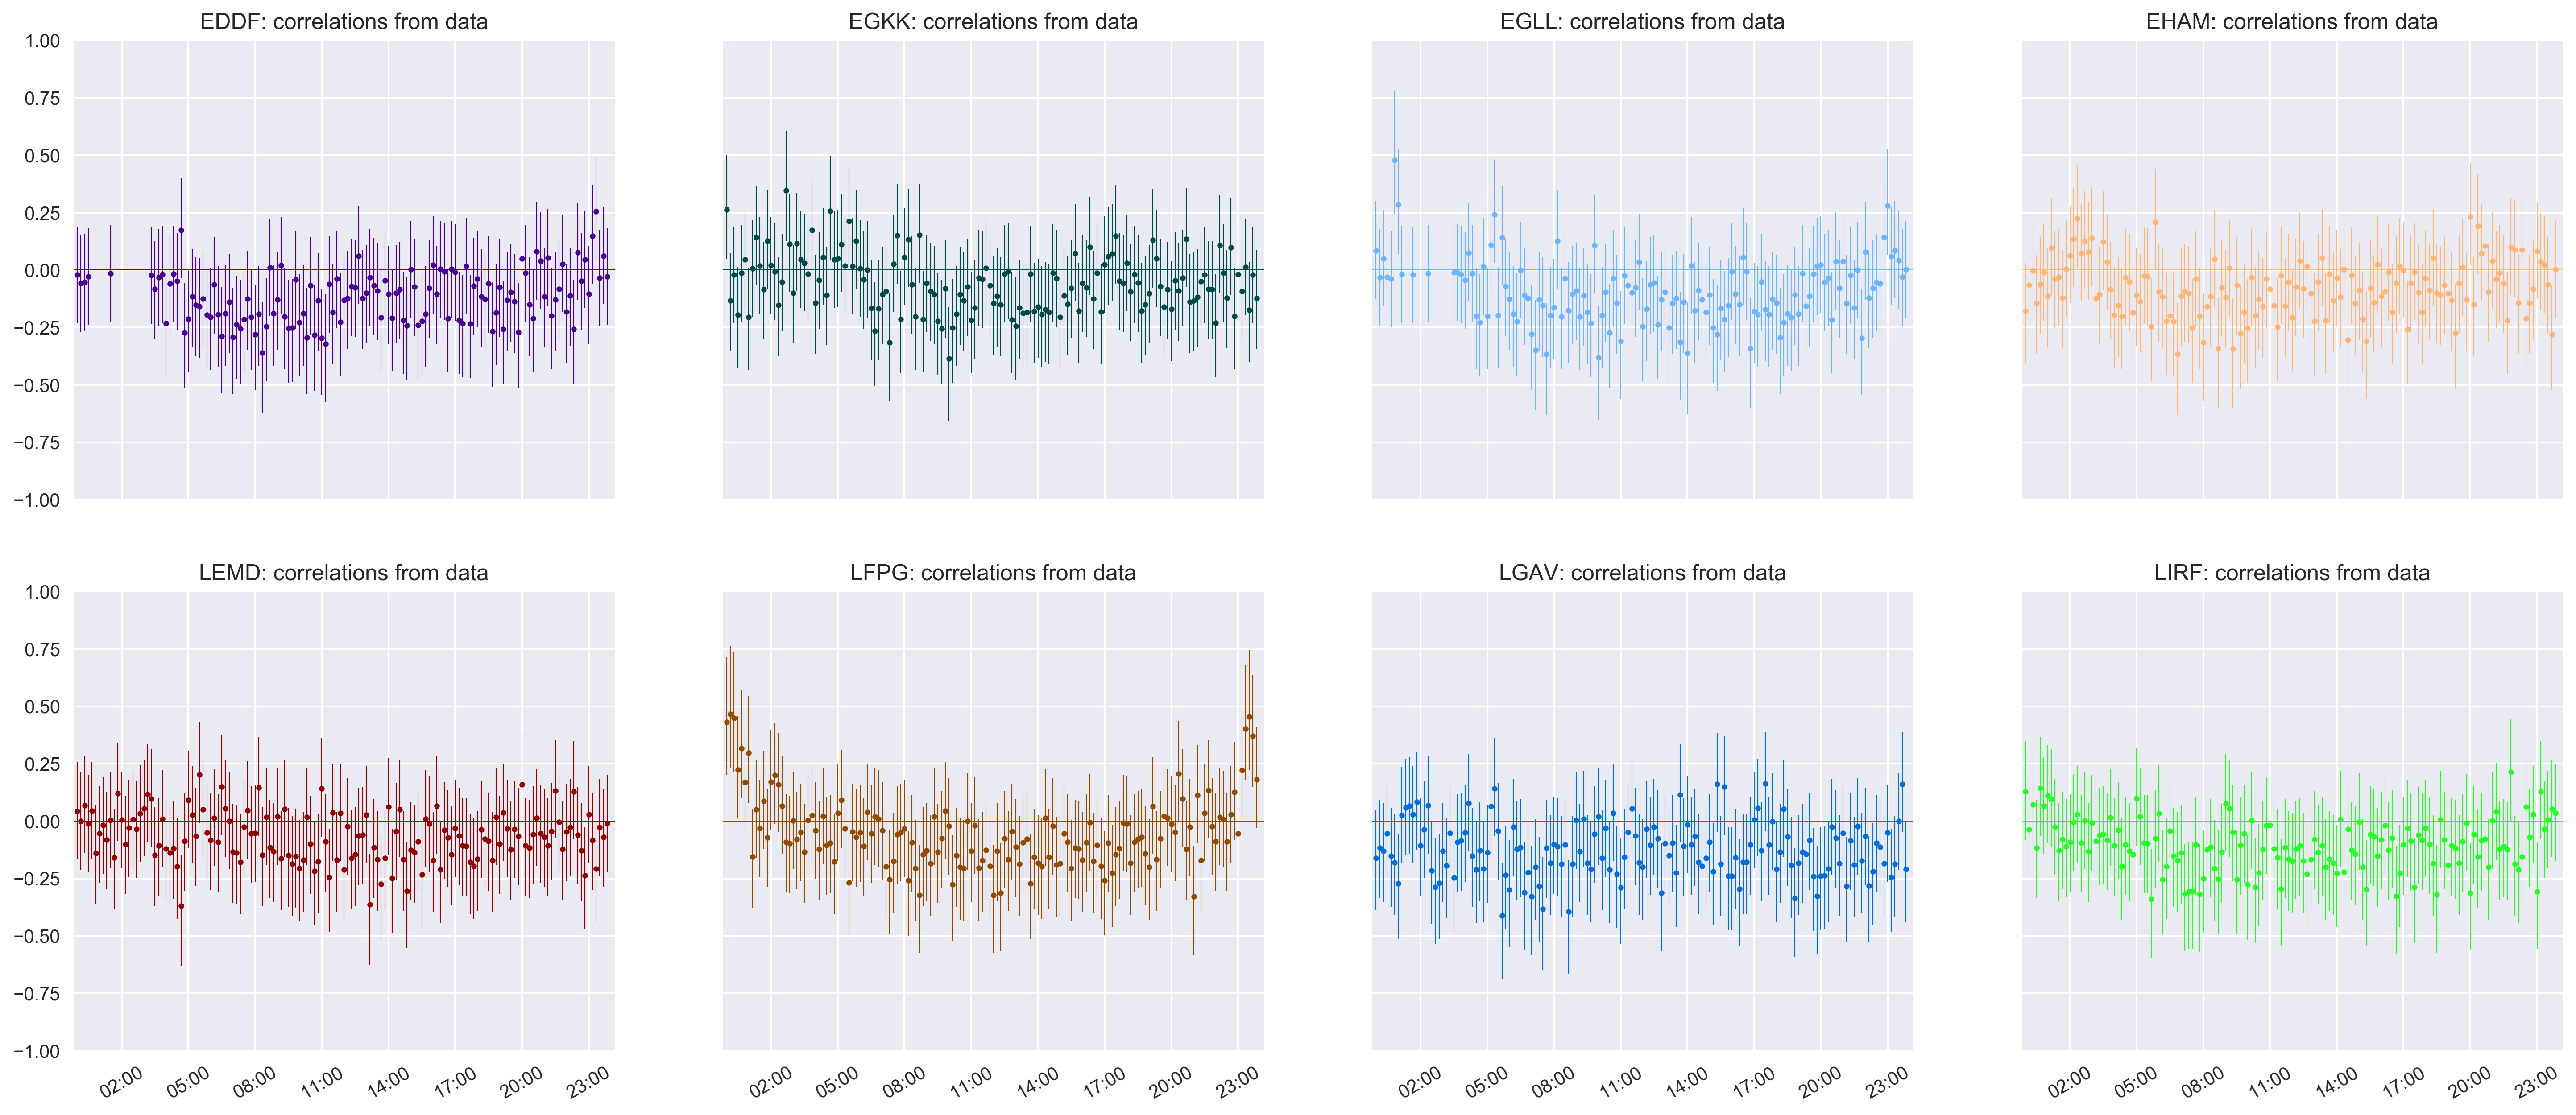
\includegraphics[width=.6\textwidth]{correlations_psra}
      \end{alertblock}
  \end{frame}

  \begin{frame}[t]\frametitle{PSRA-like arrivals inherit the correlation structure from M1}
      \begin{alertblock}{Correlations from M1 data}
        \centering
        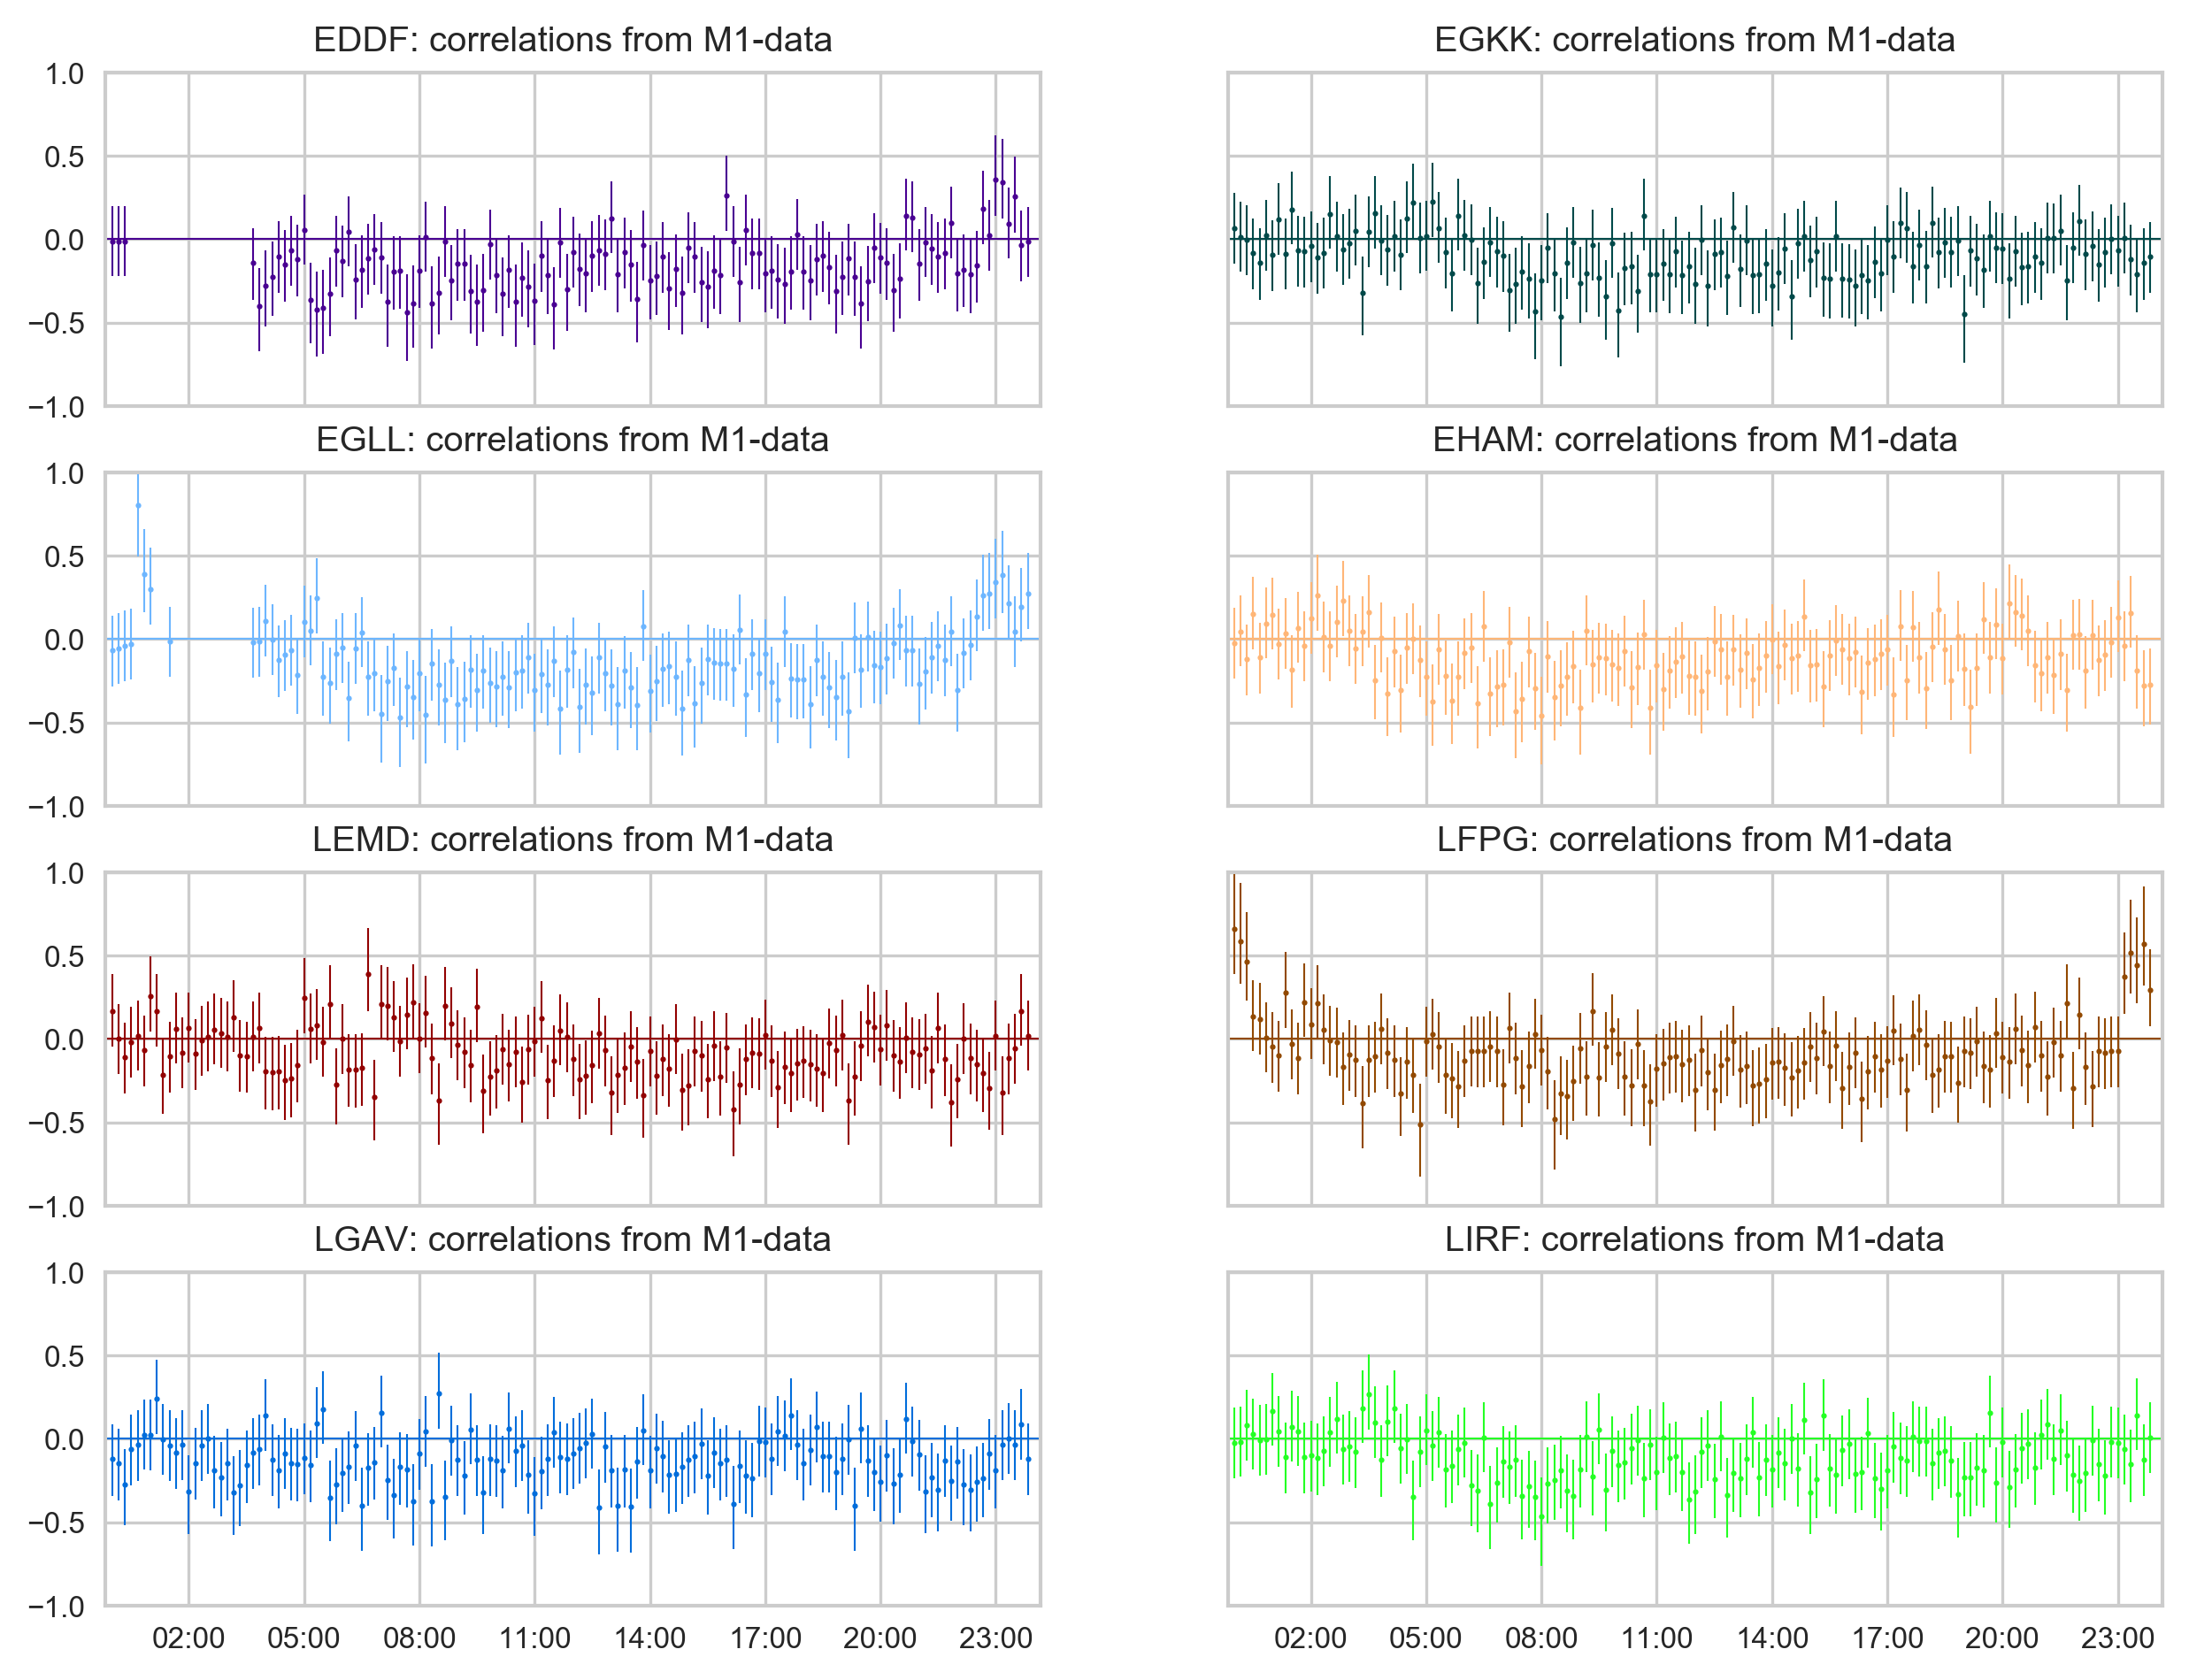
\includegraphics[width=.6\textwidth]{correlations_m1}
      \end{alertblock}
  \end{frame}

  \begin{frame}[t]\frametitle{Comparison of daily average arrivals}
      \centering
      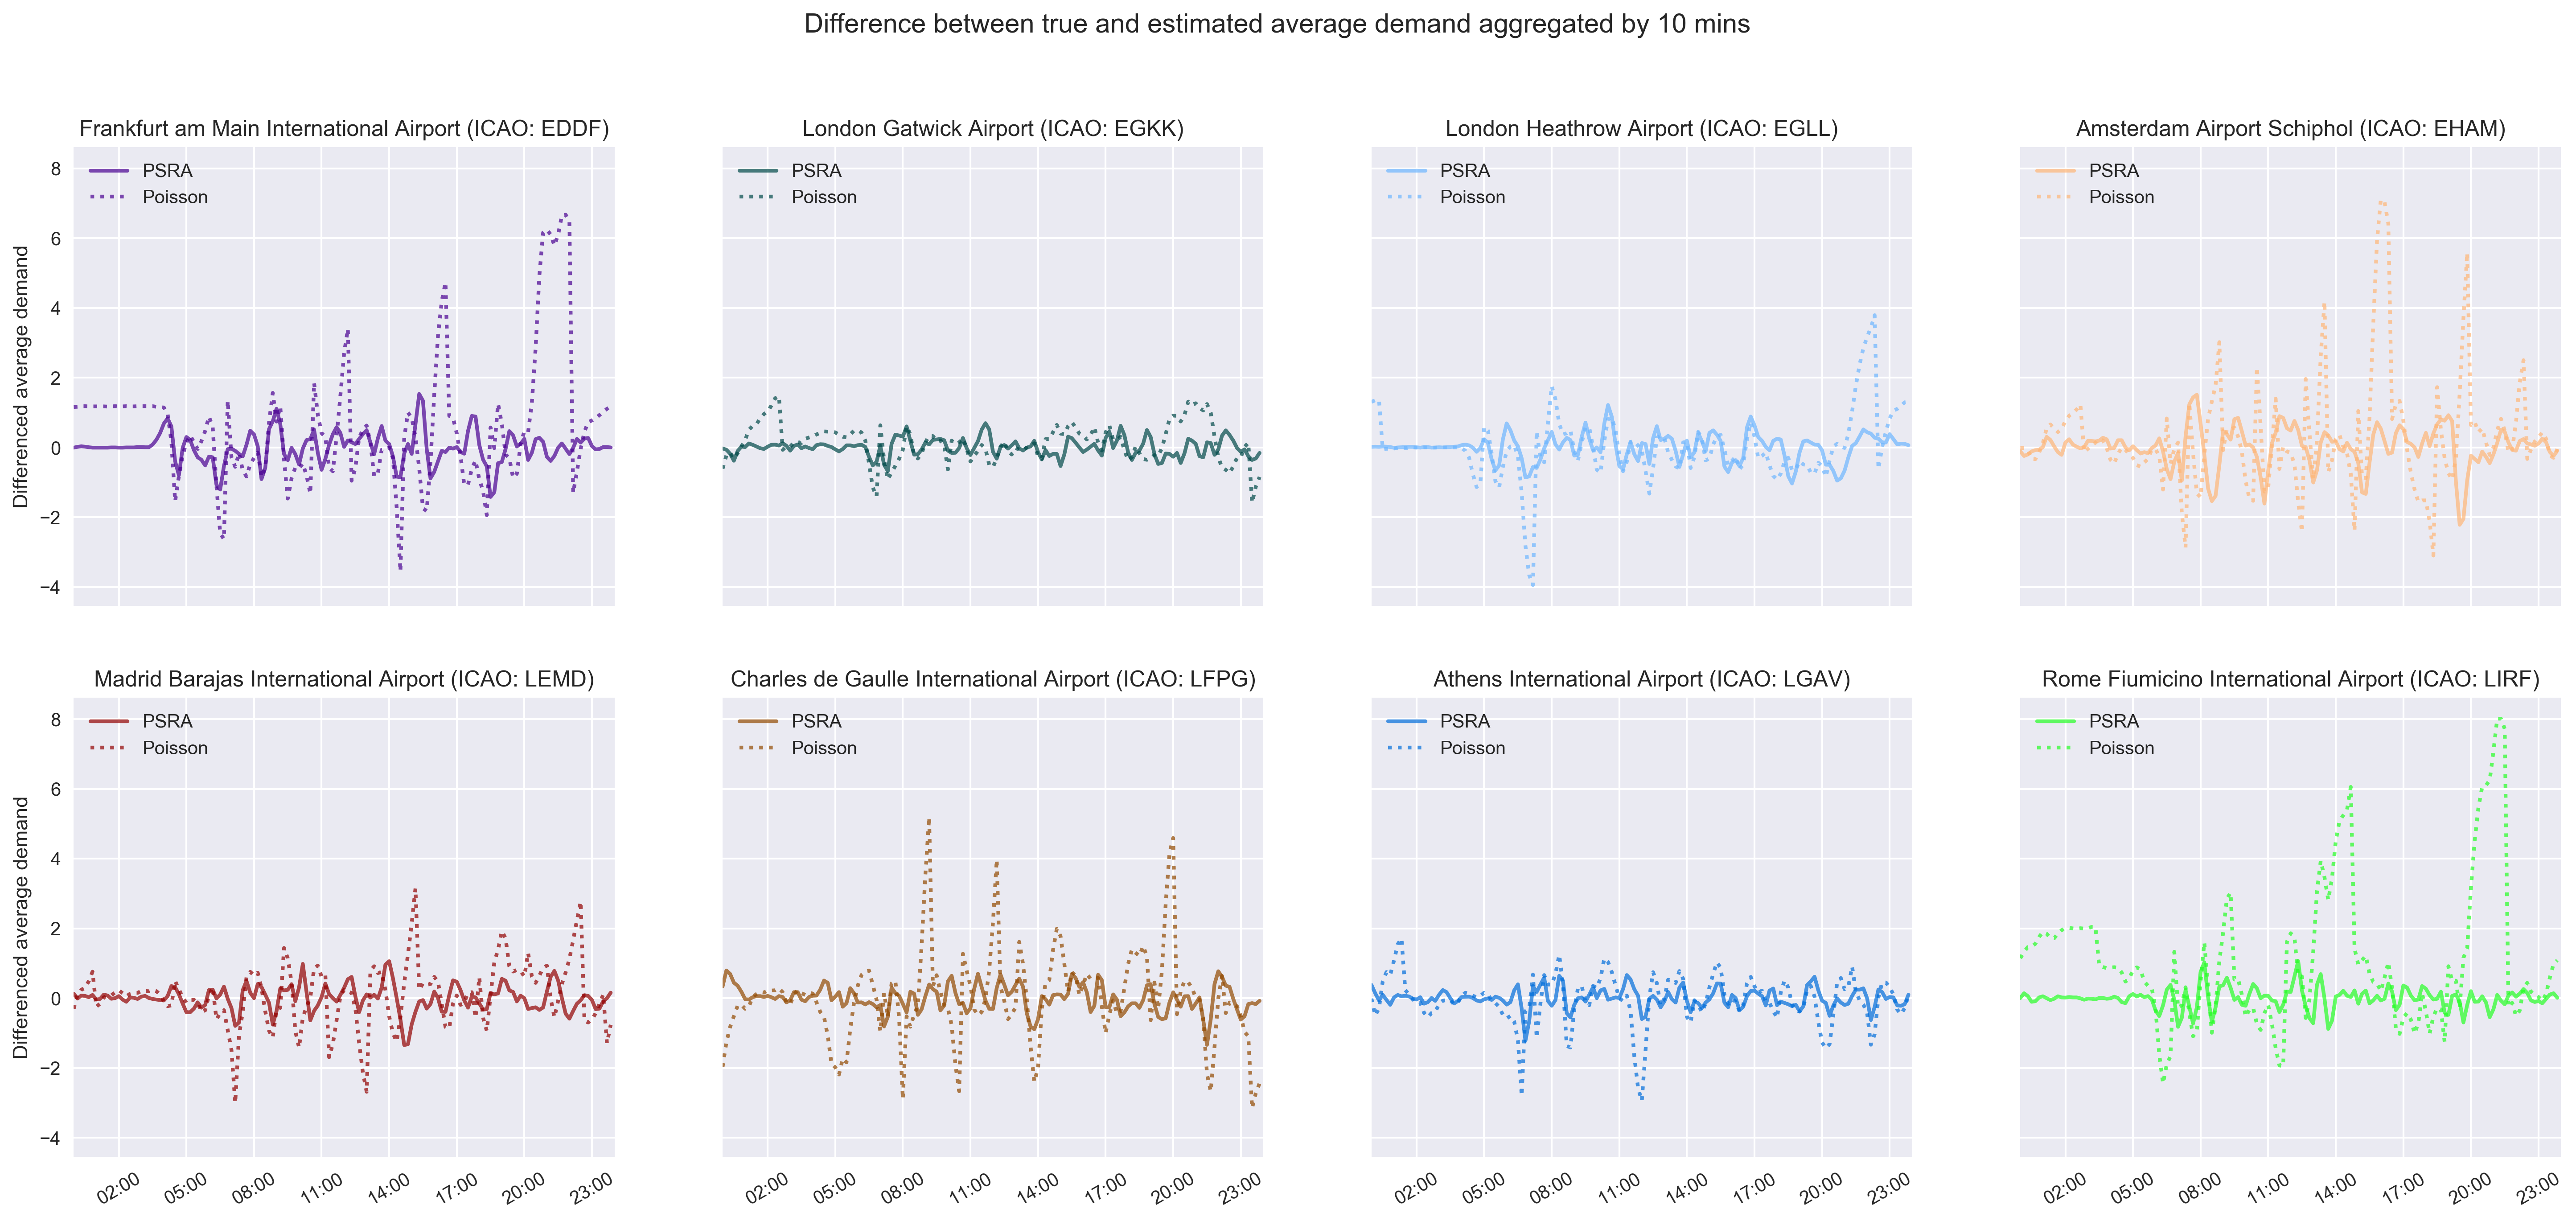
\includegraphics[width=.75\textwidth]{mean_simul_arrivals}
  \end{frame}

  \begin{frame}[t]\frametitle{Conclusions}
    Gigi
  \end{frame}

\end{document}
